\subsection{Design av Grafdatabase}
Her brukte vi datasettet "Government Types of the World" fra Kaggle: https://www.kaggle.com/janzasadny/rulers-elections-and-irregular-governance

\subsubsection{Representasjon av nodene og relasjonene mellom de}
\FigureCounter
\begin{figure}[H]
  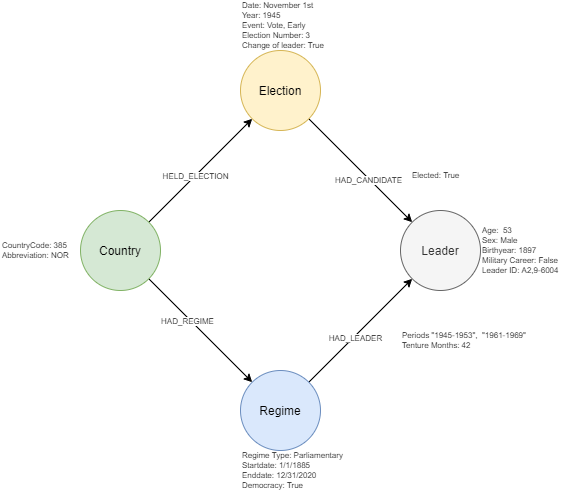
\includegraphics[scale=1]{images/milepael4/graph_database_base.drawio.png}
\end{figure}

\subsubsection{Hvorfor grafdatabase?}
Vi tenkte at grafdatabase er godt egnet for å se hvilke styringsmåter forskjellige land har. Det gir 
også en god oversikt over hvilke ledere som har styrt hvor, og eventuelt om de har styrt andre 
steder. Siden det ikke er for omfattende informasjon om hver node, kan de lett lagres som 
egenskaper. Det gjør det også lett å få oversikt på presteringen av hver leder og hvert land.

\subsubsection{Operasjoner}

\subsubsection{Hvordan eksisterende data oppdateres}
I vår løsning for grafdatabaser lagres ikke komponentene direkte i databasen som objekter, men blir 
heller laget via queries. Derfor er det ikke samme behov for et rådata-objekt for å oppdatere disse 
komponenetene. Måten vi tenker at dette gjøres er at brukeren oppretter en ny node som skal 
plottes inn i databasen. For eksempel, kan brukeren opprette en ny leder-node med tilhørende 
properties, og det er denne som sendes til databasen.

\subsection{Dataobjekter}
% Aggregering 1 %
\subsubsection{Regi}
Denne framstiller populariteten blant de forskjellige Regjeringstypene ved å telle opp land.

\FigureCounter
\begin{figure}[H]
  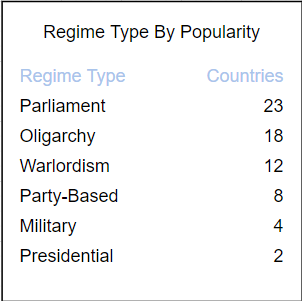
\includegraphics[scale=1]{images/milepael4/regimeTypeByPopularity.png}
\end{figure}

\textbf{Pseudo-Kode}
\begin{enumerate}
  \item Register each field from user input
  \item Save data as an object
  \item Post object to database
\end{enumerate}